As a new idea, this study introduces the concept of trustless transport which replaces the need of central intermediation of supply and demand. We propose a mechanism which punishes hostile actors automatically resulting in no conflict resolution required from central entities. \par
In our scenario seen at figure \ref{fig:1 main overview}, we assume that the service consumer \textit{A} wants to send an physical asset to the endpoint actor \textit{B}, and that the asset payment between them already took place. Let the service provider \textit{C}, \textit{A} and \textit{B} all have an ECDSA key pair \textit{\{PK, SK\}}. \par
The scenario starts of with \textit{A} creating a request for transport minimally containing {\textit{PKb}}, \textit{Loc b} and \textit{Loc A}. This order in the orderbook is accepted by \textit{C} which then signs \textit{\{PKc, SKc\}} a UTXO \textit{tx1} containing the equivalent cost of the asset or more to 2/2 multisig address of \textit{\{PKb, PKc\}}. \par

\begin{figure}[h]
\centering
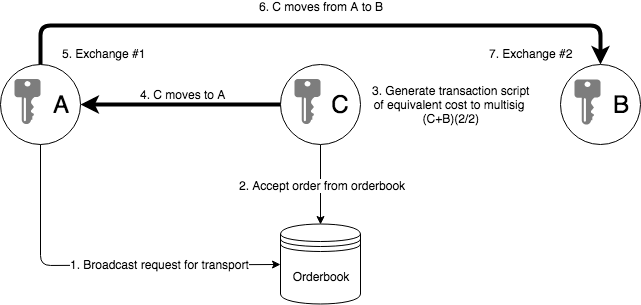
\includegraphics[width=1\textwidth]{images/main.png}
\caption{Overview test scenario}
\label{fig:1 main overview}
\end{figure}

Actor \textit{C} moves to the physical location of actor \textit{A} bringing the signed transaction script. As illustrated with figure \ref{fig:2 first exchange}, upon \textit{C} arriving at \textit{A} the first exchange can take place. \par
\textit{C} innitiates the exchange by giving \textit{A} the transaction script of \textit{tx1}. Upon receiving the transaction script \textit{A} generates and signs \textit{\{PKa, SKa\}} UTXO \textit{tx2} containing the tansport cost of the asset to 2/2 multisig address of \textit{\{PKb, PKc\}}. The service consumer actor \textit{A} now broadcasts \textit{tx1}, \textit{tx2} and digital asset ownership from \textit{A} to \textit{B}. Before \textit{tx1} and \textit{tx2} get broadcasted \textit{A} and \textit{C} can individually verify if the signed transactions actually contain what they should. After waiting the appropiate confirmations the physical asset gets exchanged from \textit{A} to \textit{B}.

\begin{figure}[h]
\centering
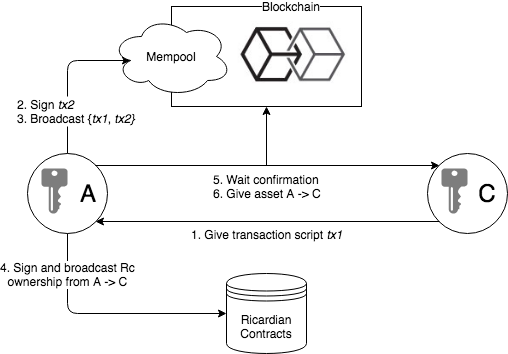
\includegraphics[width=1\textwidth]{images/exchange_01.png}
\caption{Exchange between A and C}
\label{fig:2 first exchange}
\end{figure}

 When \textit{C} recieves the asset he is the custodian and will move the asset to the endpoint \textit{Loc B}. Upon \textit{C} arriving at \textit{Loc B} the second exchange takes place which consist out of the following steps:

\begin{enumerate}
  \item \textit{B} signs \textit{\{PKb, SKb\}} two UTXO's \textit{\{tx1, tx2\}} containing the (equivalent cost + tansport cost) of 2/2 multisig address of \textit{\{PKb, PKc\}} to address of \textit{C} \textit{\{PKc\}} and give this to \textit{C}
  \item Exchange asset \textit{C} to \textit{B}
\end{enumerate}

At the end of the second exchange actor \textit{C} now owns the transaction script containing the (equivalent cost + tansport cost) of 2/2 multisig address of \textit{\{PKb, PKc\}} to address of \textit{C} \textit{\{PKc\}} and can sign the transaction with his own keypair whenever he wants to redeem the funds.
